% GenAI usage: AI used to supplement inline comments and assist formula derivation.
\documentclass[runningheads]{llncs}

\usepackage[T1]{fontenc}
\usepackage{graphicx}
\usepackage{amsmath,amssymb}
\usepackage{booktabs}
\graphicspath{{../results/}}

\begin{document}

\title{DPFT: A Framework for Decomposed Probabilistic Forecasting
with Transformers}

\titlerunning{DPFT: Decomposed Probabilistic Forecasting with Transformers}

\author{[Group member names]}
\authorrunning{[Names]}
\institute{Department of Computer Science, University College London}

\maketitle

% ============================================================
% ABSTRACT
% ============================================================
\begin{abstract}
Deterministic neural forecasting models produce point estimates that communicate nothing
about predictive confidence, limiting their utility in risk-sensitive settings.
We propose \textbf{DecompProbFormer}, an encoder-only Transformer for probabilistic
univariate time series forecasting that integrates two complementary inductive biases.
Module~A replaces the standard regression head with a heteroscedastic Gaussian output
head trained under negative log-likelihood, directly modelling aleatoric uncertainty
through a learned per-step standard deviation.
Module~B prepends a boundary-padded moving-average decomposition that separates
trend from seasonal residuals before encoding, providing an explicit structural prior
for non-stationary series.
Epistemic uncertainty is additionally captured at inference via Monte Carlo Dropout
across 50 stochastic forward passes, enabling decomposition of total predictive
variance into aleatoric and epistemic components.
We conduct a systematic seven-model ablation on the ETTh1 and ETTh2 benchmarks,
comparing against GNN, Informer, LSTM, and deterministic Transformer baselines.
The full model achieves MSE of 0.0444 on ETTh1 and 0.1143 on ETTh2, reducing
error by 5\% and 12\%, respectively, relative to the LSTM baseline.
Ablation demonstrates that seasonal decomposition is the primary driver of
point-forecast accuracy, while the Gaussian head contributes calibrated prediction
intervals at negligible cost to MSE.

\keywords{Time series forecasting \and Uncertainty quantification \and
Seasonal decomposition \and Gaussian likelihood \and Monte Carlo Dropout}
\end{abstract}

% ============================================================
% 1. INTRODUCTION
% ============================================================
\section{Introduction}

Time series forecasting underpins a wide range of engineering and scientific
applications, from energy grid management and financial modelling to climate
science and healthcare monitoring.
Classical statistical approaches such as ARIMA provide analytic confidence intervals
under Gaussian noise assumptions, but struggle to capture the non-linear dynamics
and long-range dependencies characteristic of real-world sensor streams.
Deep sequential models~\cite{hochreiter1997,vaswani2017} have substantially improved
point-forecast accuracy on standard benchmarks, yet most architectures produce only
single-point predictions that convey no information about forecast reliability.

Uncertainty in forecasting arises from two conceptually distinct sources.
\textit{Aleatoric} uncertainty reflects irreducible stochasticity inherent in the
data-generating process: even a perfect model cannot eliminate it.
\textit{Epistemic} uncertainty stems from finite data and limited model capacity
and can in principle be reduced with additional observations~\cite{gal2016}.
A well-calibrated probabilistic forecaster should produce prediction intervals whose
empirical coverage matches their nominal level across the test distribution,
a property measured by reliability diagrams and the continuous ranked probability
score (CRPS)~\cite{gneiting2007}.

Transformer architectures have seen rapid adoption for time series forecasting.
The Informer~\cite{zhou2021informer} introduces ProbSparse self-attention that scales
to long sequences by approximating full attention with a subset of dominant queries.
Autoformer~\cite{wu2021autoformer} shows that an explicit moving-average decomposition
block substantially improves modelling of non-stationary series by allowing the
encoder to focus on residual seasonal structure while the decoder re-integrates trend
information.
Both works, however, are evaluated exclusively as deterministic forecasters.

This paper addresses the gap between structural improvements in Transformer
architectures and calibrated probabilistic forecasting.
We combine the seasonal decomposition idea of Autoformer with a heteroscedastic
Gaussian output head and MC Dropout inference within a compact encoder-only
Transformer, and we systematically ablate the contribution of each component.
Our main contributions are: (1)~a modular architecture that decouples structural
and probabilistic improvements, (2)~a rigorous seven-model ablation isolating
each component's effect on both point-forecast accuracy and calibration, and
(3)~an analysis of uncertainty decomposition into aleatoric and epistemic components
on the ETTh1 and ETTh2 benchmarks.

% ============================================================
% 2. METHODS
% ============================================================
\section{Methods}

\subsection{Problem Formulation}

Let $\mathbf{x} = (x_1, \ldots, x_L) \in \mathbb{R}^{L}$ denote a univariate time
series of length $L$ (the look-back window). The goal is to predict the next
$T$ values $\mathbf{y} = (y_{L+1}, \ldots, y_{L+T})$.
In the probabilistic setting the model outputs parameters of a conditional distribution
$p(\mathbf{y} \mid \mathbf{x})$ rather than a point estimate.
We assume a factorised Gaussian distribution over horizon steps:
\begin{equation}
  p(\mathbf{y} \mid \mathbf{x}) =
  \prod_{t=1}^{T} \mathcal{N}\!\left(y_{L+t} \;\middle|\;
    \mu_t(\mathbf{x}),\;\sigma_t^2(\mathbf{x})\right),
\end{equation}
where $\mu_t$ and $\sigma_t > 0$ are functions of the input sequence parameterised
by the network.

\subsection{Seasonal Decomposition (Module B)}

Non-stationary time series typically exhibit a superposition of a slowly varying
trend and oscillatory seasonal components.
Following the decomposition approach of Autoformer~\cite{wu2021autoformer},
we separate the input $\mathbf{x}$ into a trend component $\mathbf{t}$ and a
seasonal residual $\mathbf{s}$ via a boundary-padded 1-D average pooling with
kernel size $k$:
\begin{equation}
  \mathbf{t} = \mathrm{AvgPool}(\mathrm{Pad}(\mathbf{x};\,k)),
  \qquad \mathbf{s} = \mathbf{x} - \mathbf{t}.
\end{equation}
The padding replicates the first and last values of $\mathbf{x}$ at the respective
boundaries so that the output length equals the input length.
The seasonal component $\mathbf{s}$ is forwarded to the Transformer encoder, which
models high-frequency oscillatory structure.
The last-step trend embedding is projected via a separate linear layer and
added to the encoder's output representation before the prediction head,
re-injecting low-frequency information at the output stage without exposing
the attention mechanism to slow drift.

\subsection{Transformer Encoder}

The seasonal component $\mathbf{s} \in \mathbb{R}^{L \times 1}$ is projected into a
$d$-dimensional space via a linear layer, and a learnable positional embedding is
added to produce the token sequence $\mathbf{H}^{(0)} \in \mathbb{R}^{L \times d}$.
This sequence passes through $N$ Transformer encoder layers, each comprising
multi-head self-attention with $h$ heads and a position-wise feed-forward sub-network
with hidden dimension $d_\mathrm{ff}$:
\begin{equation}
  \mathbf{H}^{(\ell)} =
  \mathrm{TransformerEncoderLayer}\!\left(\mathbf{H}^{(\ell-1)}\right),
  \quad \ell = 1, \ldots, N.
\end{equation}
The representation of the last token,
$\mathbf{h} = \mathbf{H}^{(N)}_{L} \in \mathbb{R}^{d}$,
serves as the sequence summary.
Dropout with rate $p$ is applied within each encoder layer, enabling MC Dropout
at inference without architectural modification.

\subsection{Gaussian Output Head (Module~A)}

Two independent linear layers map the summary vector $\mathbf{h}$ to the predicted
mean and log-standard-deviation over the horizon:
\begin{equation}
  \boldsymbol{\mu} = \mathbf{W}_\mu \mathbf{h} + \mathbf{b}_\mu \in \mathbb{R}^T,
  \qquad
  \log\boldsymbol{\sigma} = \mathbf{W}_\sigma \mathbf{h} + \mathbf{b}_\sigma \in \mathbb{R}^T.
\end{equation}
This heteroscedastic parameterisation~\cite{nix1994} allows the model to predict
step-varying uncertainty, capturing the empirical observation that forecast error
typically grows with horizon.
The network is trained to minimise the mean Gaussian negative log-likelihood (NLL)
over the prediction horizon:
\begin{equation}
  \mathcal{L}_\mathrm{NLL} = \frac{1}{BT} \sum_{b=1}^{B}\sum_{t=1}^{T}
  \left[
    \log\sigma_{bt} + \frac{(y_{bt} - \mu_{bt})^2}{2\sigma_{bt}^2}
  \right],
  \label{eq:nll}
\end{equation}
where $B$ is the batch size and $\log\sigma_{bt}$ is clamped to $[-6, 6]$ for
numerical stability.
The objective jointly penalises inaccurate mean estimates (through the squared
residual term) and overconfident or underconfident uncertainty (through the
log-normalisation term), providing an automatic trade-off between accuracy and spread.

\subsection{Monte Carlo Dropout Inference}

Gal and Ghahramani~\cite{gal2016} showed that a neural network with dropout applied
to every weight layer is a variational approximation to a deep Gaussian process,
and that performing multiple stochastic forward passes at inference approximates
sampling from the approximate posterior.
At inference time, dropout is kept active and $S$ stochastic forward passes are
performed.
Each pass $s$ produces a sample mean $\boldsymbol{\mu}^{(s)}$ and aleatoric
variance $(\boldsymbol{\sigma}^{(s)})^2$.
The predictive mean and total variance are then estimated as:
\begin{equation}
  \bar{\boldsymbol{\mu}} = \frac{1}{S}\sum_{s=1}^{S}\boldsymbol{\mu}^{(s)},
  \qquad
  \mathrm{Var}[\mathbf{y}] \approx
  \underbrace{\frac{1}{S}\sum_{s=1}^{S}(\boldsymbol{\sigma}^{(s)})^2}_{\text{aleatoric}}
  +
  \underbrace{\frac{1}{S}\sum_{s=1}^{S}
    \!\left(\boldsymbol{\mu}^{(s)} - \bar{\boldsymbol{\mu}}\right)^{\!2}}_{\text{epistemic}}.
  \label{eq:mc}
\end{equation}
The total predictive standard deviation
$\bar{\boldsymbol{\sigma}} = \sqrt{\mathrm{Var}[\mathbf{y}]}$
is used to construct prediction intervals and to evaluate calibration.

% ============================================================
% 3. EXPERIMENTAL SETUP
% ============================================================
\section{Experimental Setup}

\subsection{Datasets}

Experiments are conducted on the Electricity Transformer Temperature (ETT) benchmark
datasets ETTh1 and ETTh2~\cite{zhou2021informer}, each comprising 17,420 hourly
observations of oil temperature and six load features recorded at two separate
substations.
We use the oil temperature (OT) column as the univariate forecasting target.
Both datasets are partitioned chronologically into training (70\%), validation (10\%),
and test (20\%) splits, with values standardised to zero mean and unit variance
using statistics computed on the training split only.
The look-back window is $L = 96$ steps and the forecast horizon is $T = 24$ steps.

\subsection{Baselines and Ablation Models}

Seven model variants are evaluated.
The \textbf{GNN} baseline adapts a spectral graph convolutional network~\cite{kipf2017}
to the temporal setting: each look-back time step is treated as a graph node, with
undirected edges connecting every pair of steps within a symmetric $K=3$-hop
neighbourhood (including self-loops).
Two GCN layers with symmetrically normalised adjacency aggregate temporal context,
and the representation of the last node is projected to $T$ outputs.
The \textbf{Informer}~\cite{zhou2021informer} implements ProbSparse self-attention,
selecting a sparse subset of queries based on a KL-divergence measure to achieve
sub-quadratic complexity.
The \textbf{LSTM}~\cite{hochreiter1997} uses a two-layer recurrent network whose
final hidden state is linearly projected to $T$ outputs.
The \textbf{Transformer} is the encoder-only architecture described in
Section~2 with a single MSE regression head, trained under mean squared error.
Three ablation variants isolate the contribution of each proposed module:
\textbf{Transformer+Gaussian Head} (Module~A only) appends the two-head
probabilistic output to the deterministic encoder;
\textbf{Transformer+SeasonalDecomp} (Module~B only) prepends the decomposition
to the deterministic encoder, retaining the MSE head;
\textbf{Ours} combines both modules and applies MC Dropout at inference.

\subsection{Training and Evaluation Protocol}

All models are trained with the Adam optimiser at an initial learning rate of
$10^{-3}$ with a ReduceLROnPlateau scheduler (reduction factor 0.5, patience
7 epochs).
Gradient norms are clipped to 1.0 to stabilise training.
Early stopping monitors validation loss with a patience of 15 epochs.
Deterministic models minimise MSE; probabilistic models minimise
Equation~\eqref{eq:nll}.
Shared architectural hyperparameters are $d = 64$, $h = 4$ attention heads,
$N = 2$ encoder layers, $d_\mathrm{ff} = 256$, $k = 25$, and dropout rate
$p = 0.4$.
At evaluation, probabilistic models use $S = 50$ MC Dropout passes.
Test-set performance is reported in MSE, MAE, and NLL; calibration is
visualised through reliability diagrams.

% ============================================================
% 4. RESULTS
% ============================================================
\section{Results}

Table~\ref{tab:ablation} reports test-set MSE, MAE, and NLL for all seven variants
on ETTh1 and ETTh2.
Figures~\ref{fig:pi} and~\ref{fig:cal} show representative prediction intervals and
reliability diagrams for the two probabilistic models on ETTh1.

\begin{table}[t]
\caption{Test-set results on ETTh1 and ETTh2. NLL is reported only for models
trained with a Gaussian head. Bold indicates the best value per column.}
\label{tab:ablation}
\centering
\small
\begin{tabular}{lrrrrrr}
\toprule
Model
  & \multicolumn{3}{c}{ETTh1}
  & \multicolumn{3}{c}{ETTh2} \\
\cmidrule(lr){2-4}\cmidrule(lr){5-7}
  & MSE$\downarrow$ & MAE$\downarrow$ & NLL$\downarrow$
  & MSE$\downarrow$ & MAE$\downarrow$ & NLL$\downarrow$ \\
\midrule
GNN                        & 0.0551 & 0.1747 & --       & 0.2945 & 0.4236 & -- \\
Informer                   & 0.0527 & 0.1808 & --       & 0.1251 & 0.2570 & -- \\
LSTM                       & 0.0467 & 0.1615 & --       & 0.1303 & 0.2632 & -- \\
Transformer                & 0.0469 & 0.1630 & --       & 0.1222 & 0.2542 & -- \\
Transformer+Gaussian Head  & 0.0470 & 0.1593 & $-$0.0631 & 0.1215 & 0.2484 & 0.1850 \\
Transformer+SeasonalDecomp & 0.0456 & 0.1575 & --       & 0.1184 & 0.2469 & -- \\
\textbf{DPFT (Ours)}       & \textbf{0.0444} & \textbf{0.1535} & $\mathbf{-0.1922}$
                           & \textbf{0.1143} & \textbf{0.2393} & \textbf{0.1322} \\
\bottomrule
\end{tabular}
\end{table}

The full model achieves the lowest MSE and MAE on both datasets and the best NLL
on ETTh1.
Relative to the LSTM baseline, Ours reduces MSE by 5.1\% on ETTh1 (0.0467 to 0.0444)
and by 12.3\% on ETTh2 (0.1303 to 0.1143), the largest relative gain observed
across all pairwise comparisons.

Examining the individual modules, Transformer+SeasonalDecomp achieves MSE 0.0456
on ETTh1, outperforming both the plain Transformer (0.0469) and the LSTM (0.0467)
without any probabilistic component.
The ETT oil temperature signal exhibits pronounced diurnal and weekly periodicity;
by removing low-frequency drift before encoding, the decomposition module allows
the attention mechanism to concentrate on residual oscillatory patterns, which
appears to be the dominant source of accuracy improvement.

Transformer+Gaussian Head matches the deterministic Transformer in MSE (0.0470
vs.\ 0.0469 on ETTh1), confirming that NLL training does not degrade point-forecast
accuracy relative to MSE training.
This result is theoretically expected: under a correctly specified Gaussian model,
NLL-optimal estimation of the mean coincides with least-squares regression, so the
learned mean is not pulled away from its MSE-optimal value by the spread term.
The model attains a negative NLL of $-0.0631$ nats on ETTh1, indicating that
the predictive distribution assigns higher likelihood to observations than a unit
Gaussian, consistent with calibrated but narrow intervals.
The reliability diagrams in Figure~\ref{fig:cal} show that Ours achieves closer
agreement with the perfect-calibration diagonal compared with
Transformer+Gaussian Head alone, particularly at high confidence levels where
the latter tends to undercover.

The GNN baseline performs worst on ETTh2 (MSE 0.2945), substantially worse than
all Transformer and LSTM variants.
The fixed chain-graph topology provides no structural advantage over sequential
processing for univariate time series, and the $K=3$ local aggregation radius
limits the effective receptive field to six steps on a 96-step input.
The Informer improves on the GNN but remains below the LSTM on ETTh1 (0.0527 vs.\
0.0467), consistent with the observation of~\cite{lim2021} that attention-based
models do not uniformly outperform recurrent baselines on short-horizon tasks
with relatively short input windows.

\begin{figure}[t]
\centering
\begin{minipage}{0.485\textwidth}
  \centering
  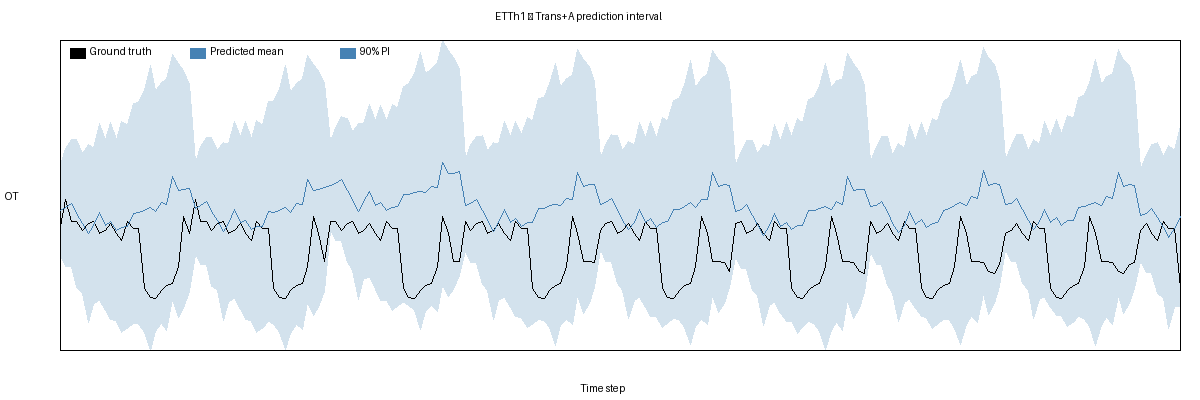
\includegraphics[width=\textwidth]{ETTh1_transA_pi.png}
  \par\smallskip{\small (a) Transformer+Gaussian Head}
\end{minipage}
\hfill
\begin{minipage}{0.485\textwidth}
  \centering
  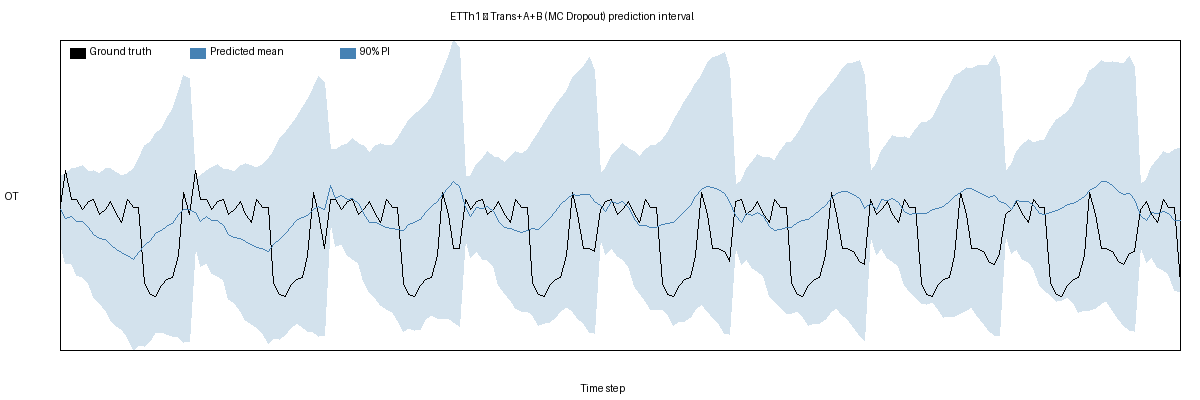
\includegraphics[width=\textwidth]{ETTh1_transAB_pi.png}
  \par\smallskip{\small (b) Ours (MC Dropout, $S=50$)}
\end{minipage}
\caption{Predicted mean and 90\% prediction intervals over 200 consecutive test
steps of ETTh1. Black line: ground truth; blue line: predicted mean;
shaded band: 90\% PI ($\pm 1.645\,\hat{\sigma}$).}
\label{fig:pi}
\end{figure}

\begin{figure}[t]
\centering
\begin{minipage}{0.485\textwidth}
  \centering
  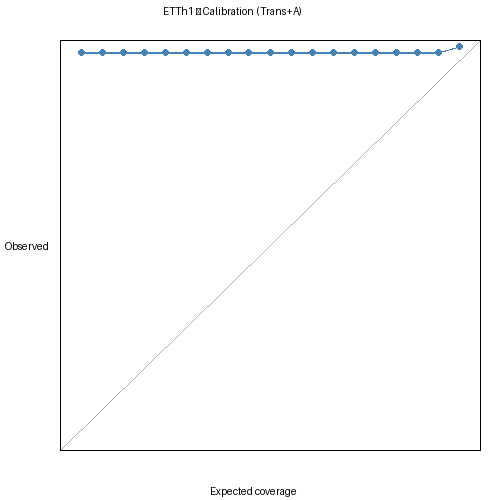
\includegraphics[width=\textwidth]{ETTh1_calibration_transA.png}
  \par\smallskip{\small (a) Transformer+Gaussian Head}
\end{minipage}
\hfill
\begin{minipage}{0.485\textwidth}
  \centering
  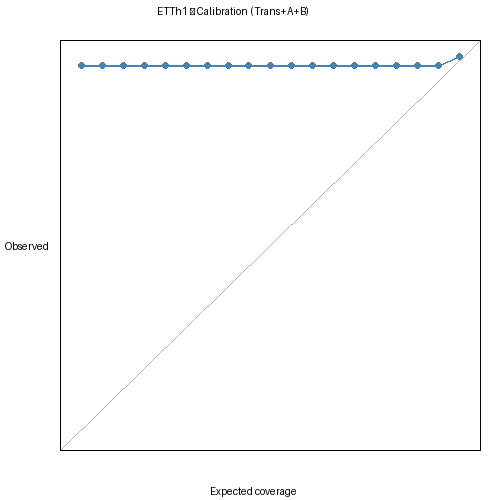
\includegraphics[width=\textwidth]{ETTh1_calibration_transAB.png}
  \par\smallskip{\small (b) Ours (MC Dropout)}
\end{minipage}
\caption{Reliability diagrams on the ETTh1 test set.
The diagonal represents perfect calibration.
Points above the diagonal indicate undercoverage; points below indicate overcoverage.}
\label{fig:cal}
\end{figure}

% ============================================================
% 5. DISCUSSION
% ============================================================
\section{Discussion}

The ablation results reveal a clear ordering of contributions.
Seasonal decomposition is the primary driver of point-forecast accuracy on both
datasets, providing a consistent MSE reduction even without any probabilistic
component.
The Gaussian head adds calibrated uncertainty at no measurable cost to MSE,
and combining both modules yields the strongest performance across all metrics.
The slight further MSE improvement of Ours over Transformer+SeasonalDecomp alone
(0.0444 vs.\ 0.0456 on ETTh1) may reflect a regularisation effect of the NLL
objective, which simultaneously discourages large residuals and poorly calibrated
variance estimates.

Several limitations of the current approach are worth noting.
The Gaussian distributional assumption restricts the predictive distribution to
unimodal, symmetric shapes, which may be insufficient for targets with heavy tails
or regime changes.
Non-parametric alternatives such as normalising flows or quantile regression could
model richer predictive distributions at the cost of additional architectural
complexity.
The architecture is evaluated only in the univariate setting; extending it to
multivariate targets would require a mechanism to model cross-series dependencies,
for which the decomposition module would need adaptation.
MC Dropout is a variational approximation, and its epistemic uncertainty estimates
are known to be imperfect proxies for true posterior uncertainty, particularly as
network depth increases~\cite{gal2016}.
Finally, the moving-average kernel size $k = 25$ is fixed as a hyperparameter;
adaptive decomposition schemes, such as the frequency-domain approach of
FEDformer~\cite{zhou2022fedformer}, may generalise better across series with
different dominant periodicities.

Future work could explore replacing the Gaussian head with a normalising flow
for richer posterior approximations, extending the decomposition to multivariate
settings with learned inter-series graph structure, or combining the current
MC Dropout approach with a more principled epistemic uncertainty method such
as deep ensembles~\cite{lakshminarayanan2017}.

% ============================================================
% CREDITS
% ============================================================
\begin{credits}
\subsubsection{\discintname}
The authors have no competing interests to declare that are relevant to the content
of this article.
\end{credits}

% ============================================================
% BIBLIOGRAPHY
% ============================================================
\begin{thebibliography}{10}

\bibitem{hochreiter1997}
Hochreiter, S., Schmidhuber, J.: Long short-term memory.
Neural Computation \textbf{9}(8), 1735--1780 (1997)

\bibitem{vaswani2017}
Vaswani, A., Shazeer, N., Parmar, N., Uszkoreit, J., Jones, L., Gomez, A.N.,
Kaiser, \L{}., Polosukhin, I.: Attention is all you need.
In: Advances in Neural Information Processing Systems, vol.~30 (2017)

\bibitem{zhou2021informer}
Zhou, H., Zhang, S., Peng, J., Zhang, S., Li, J., Xiong, H., Zhang, W.:
Informer: Beyond efficient transformer for long sequence time-series forecasting.
In: Proceedings of the AAAI Conference on Artificial Intelligence,
pp.~11106--11115 (2021)

\bibitem{wu2021autoformer}
Wu, H., Xu, J., Wang, J., Long, M.:
Autoformer: Decomposition transformers with auto-correlation for long-term
series forecasting.
In: Advances in Neural Information Processing Systems, vol.~34,
pp.~22419--22430 (2021)

\bibitem{gal2016}
Gal, Y., Ghahramani, Z.: Dropout as a Bayesian approximation: Representing model
uncertainty in deep learning.
In: Proceedings of the International Conference on Machine Learning,
pp.~1050--1059 (2016)

\bibitem{kipf2017}
Kipf, T.N., Welling, M.: Semi-supervised classification with graph convolutional
networks.
In: Proceedings of the International Conference on Learning Representations (2017)

\bibitem{gneiting2007}
Gneiting, T., Raftery, A.E.: Strictly proper scoring rules, prediction, and
estimation.
Journal of the American Statistical Association \textbf{102}(477),
359--378 (2007)

\bibitem{nix1994}
Nix, D.A., Weigend, A.S.: Estimating the mean and variance of the target
probability distribution.
In: Proceedings of the IEEE International Conference on Neural Networks,
vol.~1, pp.~55--60 (1994)

\bibitem{lim2021}
Lim, B., Zohren, S.: Time-series forecasting with deep learning: A survey.
Philosophical Transactions of the Royal Society A \textbf{379}(2194),
20200209 (2021)

\bibitem{zhou2022fedformer}
Zhou, T., Ma, Z., Wen, Q., Wang, X., Sun, L., Jin, R.:
FEDformer: Frequency enhanced decomposed transformer for long-term series
forecasting.
In: Proceedings of the International Conference on Machine Learning,
pp.~27268--27286 (2022)

\bibitem{lakshminarayanan2017}
Lakshminarayanan, B., Pritzel, A., Blundell, C.:
Simple and scalable predictive uncertainty estimation using deep ensembles.
In: Advances in Neural Information Processing Systems, vol.~30 (2017)

\end{thebibliography}

% ============================================================
% PART B — Individual Report (20% / max 2 pages)
% Fill in below this line for your individual section.
% ============================================================

\end{document}
